\documentclass[sigconf]{acmart}

\usepackage{tabularx}

%% \setcopyright{acmlicensed}
\copyrightyear{2024}
\acmYear{2024}
\setcopyright{licensedusgovmixed}\acmConference[CSCW Companion '24]{Companion of the 2024 Computer-Supported Cooperative Work and Social Computing}{November 9--13, 2024}{San Jose, Costa Rica}
\acmBooktitle{Companion of the 2024 Computer-Supported Cooperative Work and Social Computing (CSCW Companion '24), November 9--13, 2024, San Jose, Costa Rica}
\acmDOI{10.1145/3678884.3681879}
\acmISBN{979-8-4007-1114-5/24/11}

\usepackage{svg}

\begin{document}

\title{Universal Basic Philanthropy: Design and Analysis of a Grassroots Effort to Democratize Social Profit}

\author{Thien-Nam Dinh}
\email{thiennam.tnd@gmail.com}
\affiliation{%
  \institution{Token Ibis}
  \city{Albuquerque}
  \state{NM}
  \country{USA}
}

\begin{abstract}
  In democratic society, few processes are more consequential than the mechanisms for funding public goods.
  The subject of this study is one attempt to demonstrate such a mechanism: a real-world experiment to pioneer a concept called Universal Basic Philanthropy.
  In this experiment, a local nonprofit in the city of Albuquerque distributed free money to individuals to reallocate to other local nonprofits of their choosing.
  Over the course of approximately four years, the project facilitated \$145,641 over 13,812 donations from 702 people to 59 organizations.
  In this study, I use publicly available transaction data from the Albuquerque pilot project to explore the following question: how we can better understand social demand for public goods?
  Using a network approach, I characterize the organizations supported by participants in the project using three measures of graph centrality: intensity, popularity, and connectivity.
  I use natural language processing to embed, cluster, and aggregate these centrality measures at the level of causes.
  The paramount result is as follows: organizations in arts, culture, and education have a comparative advantage in the intensity of fundraising while organizations in civics, basic needs, and other causes have a comparative advantage in connectivity.
\end{abstract}

\begin{CCSXML}
<ccs2012>
   <concept>
       <concept_id>10003120.10003130.10011762</concept_id>
       <concept_desc>Human-centered computing~Empirical studies in collaborative and social computing</concept_desc>
       <concept_significance>500</concept_significance>
       </concept>
   <concept>
       <concept_id>10010405.10010455.10010461</concept_id>
       <concept_desc>Applied computing~Sociology</concept_desc>
       <concept_significance>300</concept_significance>
       </concept>
   <concept>
       <concept_id>10002951.10003227.10003233.10010519</concept_id>
       <concept_desc>Information systems~Social networking sites</concept_desc>
       <concept_significance>300</concept_significance>
       </concept>
   <concept>
       <concept_id>10010147.10010178.10010179.10003352</concept_id>
       <concept_desc>Computing methodologies~Information extraction</concept_desc>
       <concept_significance>100</concept_significance>
       </concept>
 </ccs2012>
\end{CCSXML}

\ccsdesc[500]{Human-centered computing~Empirical studies in collaborative and social computing}
\ccsdesc[300]{Applied computing~Sociology}
\ccsdesc[300]{Information systems~Social networking sites}
\ccsdesc[100]{Computing methodologies~Information extraction}

\keywords{philanthropy, network analysis, natural language processing}

\received{23 May 2024}
\received[accepted]{16 July 2024}

\maketitle

\section{Introduction}
Amid the ubiquitous reach of state and corporate power, some see the third sector---the subset of the economy that includes international non-government organizations (NGOs), domestic nonprofits, and volunteer communities---as the most promising domain for true social progress.
The notional appeal is clear: a way to fund public goods that combines the prosocial values of public government with the productive efficiency of private enterprise~\cite{etzioni1973third}.
This promise has, in part, motivated a wealth of academic research into the structural nature of philanthropic giving.
Examples of relevant work include methods to correlate donations with social networks~\cite{apinunmahakul2008social}, geographic proximity~\cite{chapman2022give}, and social media activity~\cite{korolov2016predicting}~\cite{saxton2014social}.
However, serious concerns persist over the imbalanced power dynamics of this inherently plutocratic institution~\cite{maclean2021elite}~\cite{reich2020just}.
The resulting ideological tension between charity and egalitarianism has driven interest in participatory philanthropy, a collection of approaches that emphasize more community input into the decision-making process~\cite{meyer2021walking}~\cite{hauger2023nothing}~\cite{bhati2020literature}.

One concrete approach, called \emph{Universal Basic Philanthropy} (UBP), is the subject of this research.
Under UBP, all members in some well-defined set of individuals periodically receive a dedicated stipend that they can use to donate to approved nonprofit organizations.
UBP differs from conventional philanthropy in the equitable distribution of funding power.
It differs from other participatory philanthropy models, which often involve collective voting procedures, in its prioritization of individual decision-making.
In general, UBP offers an interesting setting for several potential research directions, among them: psychological considerations of personal well-being~\cite{anik2009feeling}, sociological considerations of class dominance~\cite{silver2007disentangling}, and economic considerations of local knowledge transfer~\cite{wandel2014nonprofit}.
However, research efforts in these directions---which would require supplementary theory and data---are best left for more substantial future work.
Instead, this preliminary study seeks to break ground on a more tractable, self-contained topic: UBP as a social mechanism for computing revealed philanthropic preferences.
In principle, there are two reasons why this direction is compelling. 
Since individuals do not have to spend their own money, UBP donations are distinctively:

\begin{itemize}
  \item \textbf{Representative}: The magnitude of donations does not depend on a donor's private wealth. Consequently, influence in the UBP activity is theoretically less impacted by socioeconomic status~\cite{james2007nature}.
  \item \textbf{Deliberate}: The calculus of decision-making does not depend on personal financial sacrifice. Consequently, activity in UBP is theoretically less impacted by spontaneous impulses~\cite{bennett2009impulsive}.
\end{itemize}

In this study, I assess the first known instance of a live UBP ecosystem through the lens of revealed preference.
The target platform, a real-world pilot project set in the city of Albuquerque, New Mexico, provides public access to a complete digital record of activity.
Using this resource, I describe an end-to-end process for extracting high-level insights from low-level data.
I find that inline with focus theory, the type of social cause that binds members in an organization helps determine its network centrality~\cite{feld1981focused}.
Throughout the assessment, I augment the quantitative data with qualitative insights and speculations from my personal experience with the project.\footnote{I am a founding member and sitting board member of the operating organization. However, as a volunteer contributor, I do not have any financial conflicts of interest to disclose.}
The purpose of this commentary is only to help ground intuitions and provide context for the chosen methodologies.
The primary intended contribution of this work is a computational description of the process itself.
By documenting the design and analysis of a real-world experiment, my goal is to establish a coherent basis for future efforts.


\section{Design}
In this section, I describe the salient aspects of the Albuquerque pilot.
The project is operated by Token Ibis, an all-volunteer organization created in 2019 in Albuquerque for the sole purpose of operating the pilot.
While most of its long-term funding is provided by its board of directors, it accepts donations under its 501(c)(3) status.
Its primary service is the development and maintenance of a web application that facilitates interactions between individuals and organizations according to the UBP model.
The application software, a combination of a Django backend and ReactJS frontend, is free and open-source under the GPL-3.0 license.
Although the platform maintains some private data such as private messages and user credentials, all data used in this study is publicly available through the platform's GraphQL endpoint\footnote{\url{https://api.app.tokenibis.org/graphql/}} and permitted for research use under the organization's user agreement\footnote{\url{https://tokenibis.org/user-agreement-and-privacy-policy/}}.

Access to the application is available to all users who can (1) verify a phone number and (2) log in using a Google, Facebook, or Microsoft OAuth account.
While it is technically possible for one user to open multiple accounts in violation of the platform policy, a cursory inspection of the user pool did not reveal any overt attempts to abuse the platform in this way.
Within the application, Figure~\ref{fig:application} shows three sample screenshots of the core user experience.
Users begin on the home page, which displays their current balance.
By navigating to the nonprofit page, users can browse the list of available organizations and read a short description of their mission.
Once a user selects and allocates funds, then a donation is recorded to the public ledger.
As long as the user remains active on the application, the platform automatically additional funds at the same time every week.

\begin{figure}[H]
  \centering
  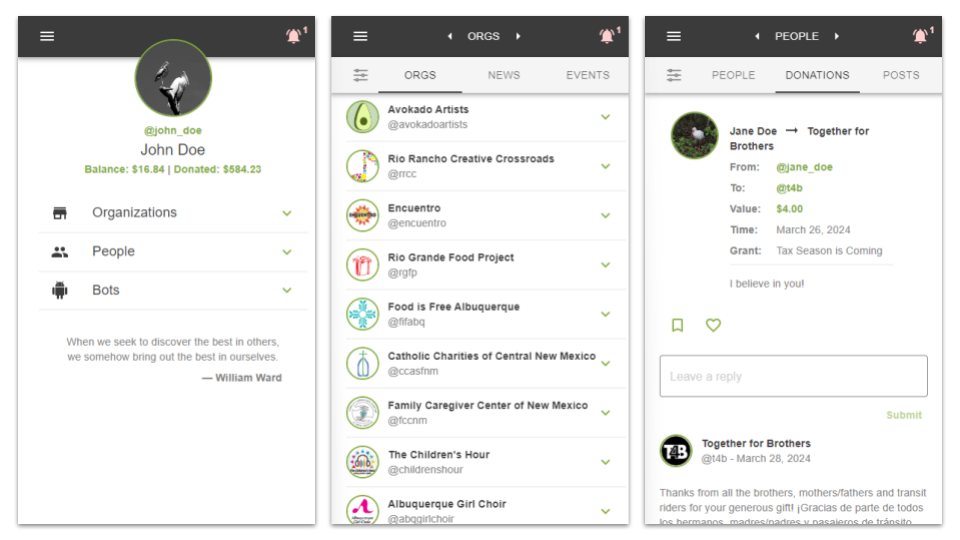
\includegraphics[width=\linewidth]{figures/application}
  \caption{Sample screenshots of the Albuquerque pilot web application (left: home screen, middle: organization list, right: donation)}
  \Description{The three screenshots convey a simple but functional Web 2.0 application.}
  \label{fig:application}
\end{figure}

In addition to the core donation workflow, the platform also supports several auxiliary activities. 

\begin{itemize}
  \item \textbf{Communication}: Users can engage in rudimentary social-media-like interactions through posts, comments, ``likes'', and private messages.
  \item \textbf{Games}: Users can participate in a set of public games---administered by on-app ``bots''---to earn more money to donate. For example, a ``vocabulary bot'' periodically rewards users who include vocabular in their donation messages that has not been used before.
  \item \textbf{Grants}: Users can deposit their own money, called grants, into the platform. These contributions are evenly distributed among all active users.
\end{itemize}

Organizations have accounts that they can use to engage with users and other organizations.
The level of engagement of each organization determines its place on the list and, therefore, its exposure to new donors.
Finally, the design of the Albuquerque pilot explicitly maintains two invariants that are relevant to this study.

\begin{itemize}

  \item \textbf{Individual Influence}: All users have equal opportunity to become influential nodes regardless.
In particular, the platform does not allow users to deposit money into their accounts.
The only mechanism for users to supplement their influence is to be active on the platform.

  \item \textbf{Organizational Exposure}: All organizations have equal opportunity to become influential nodes.
In particular, the application does not encourage users to donate to any organization based on mission type, size, or other intrinsic factors.
The only mechanism for organizations to supplement their influence is to be active on the platform.

\end{itemize}

As of May 9th, 2024, this model has facilitated the distribution of \$145,641 across 13,812 donations by 702 users to 59 organizations.
The bulk of this activity occurred over approximatley four years.
Figure~\ref{fig:graph} provides a complete picture of the network data used in this study.
Since the launch of the project, two organizations were removed for administrative reasons.
I removed the \$667.22 worth of donation activity associated with these two nonprofits from Figure~\ref{fig:graph} and all subsequent analysis.

\begin{figure}[H]
  \centering
  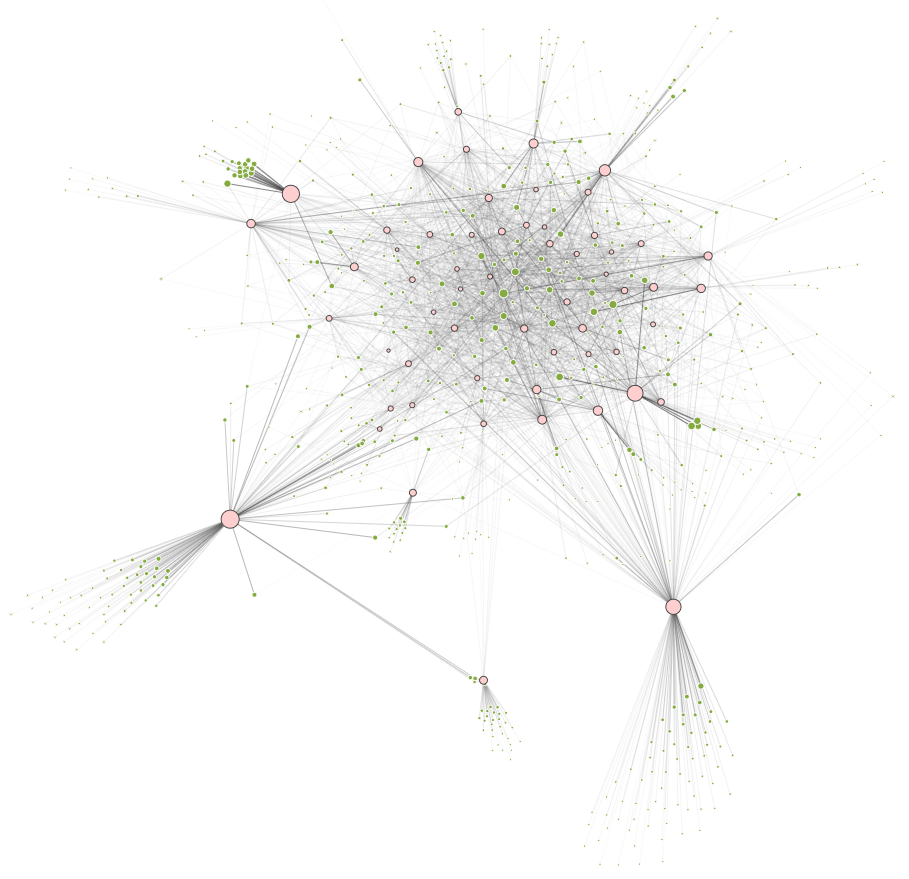
\includegraphics[width=\linewidth]{figures/network}
  \caption{Network visual of aggregate donation flow from individuals (green) to organizations (pink). The area of circles and the width and opacity of edges correspond to aggregate amounts.}
  \Description{The network is characterized by one densely connected main subgraph of individuals and organizations and several periphery hubs with one organization at the center of each hub.}
  \label{fig:graph}
\end{figure}


\section{Analysis}
In this section, I describe the methodology and results of the analysis that I performed on the data.
The overall approach is as follows.
First, I define three measures of node centrality designed to highlight specific interpretations of importance.
Next, I apply them to each organization on the platform.
Finally, I use natural language processing techniques to infer categories of causes across the ecosystem and apply the centrality measures at this higher level of abstraction.
The three centrality measures are:

\begin{itemize}
  \item \textbf{Intensity}: Intensity measures the total amount of funds that an organization raises.
    An organization's raw intensity score is the sum of the donations that it receives over its lifetime.

  \item \textbf{Popularity}: Popularity measures the funds that an organization raises while accounting for the diversity of its sources.
    An organization's raw popularity score is the sum of funds that it would hypothetically receive under a quadratic voting paradigm~\cite{lalley2018quadratic}.
    Although the choice of a quadratic adjustment is somewhat arbitrary, this distribution scheme is arguably the simplest well-known paradigm that captures both the magnitude and diversity of support for public goods.

  \item \textbf{Connectivity}: Connectivity measures the common support base that organizations share with other highly connected organizations.
    To calculate connectivity, we first need to define weighted edges between organizations.
    The procedure I use is as follows: for all pairs of organizations, find all users who have donated to both organizations.
    Represent each common user as a ``tie'' with a weight that corresponds to the geometric mean of the total amount of money the user sent to each of the two organizations.
    Finally, define the weighted edge between any two organizations as the sum of its ties.
    An organization's raw connectivity score is the eigenvector centrality calculated over this graph of weighted edges~\cite{hagberg2008exploring}.

\end{itemize}

Intuitively, these three measures correspond to objectives that different organizations might prioritize.
Intensity measures the most obvious goal: to raise as much money as possible.
However, for many organizations, the gross funding amount might be relatively less important than the number of individuals it can recruit to its cause, i.e., its popularity.  
Finally, other organizations might favor the potential for collaboration and mobilization as measured by connectivity.
These organizations would benefit from sharing many supporters with other organizations that, in turn, share supporters with still others.
All three of these measures are mutually monotonically increasing; a single marginal donation from any individual will improve the target organization's centrality in all three measures.
However, the magnitude of the increase depends on the centrality measure.
Intensity is indifferent to the identity of the donor.
Popularity considers how much the donor has previously donated to the same organization.
Connectivity considers the role of the donor in the context of the global graph structure.
In Figure~\ref{fig:graph}, these measures loosely correlate to the visual size, edge set, and geometric position of nodes.

Table~\ref{tab:org} contains a sorted list of high-centrality organizations and their relative scores.
The top three organizations in terms of intensity include an adult music choir (New Mexico Peace Choir), a professional arts support organization (Avokado Artists), and a public children's radio show (The Children's Hour).
One unifying characteristic between these organizations is that they all have dedicated members who meet regularly---performers in the first two organizations and parents of performers in the latter. 
This tight-knit, peer-based setting appears to be conducive to maintaining a group donation routine.
Meanwhile, only two organizations score higher on popularity relative to other organizations\footnote{The second organization, a youth choir (Albuquerque Girl Choir), is likely incorrectly classified.
The illusion of popularity is because it is a more recent addition to the nonprofit set. In the long term, it will likely become a high-intensity organization with a closed, dedicated support base.}.
The first, a youth mentoring program (Together for Brothers) is comprised of both regular staff and a dynamic flux of mentees.
Another organization, a crisis call center (Agora Crisis Center) has a similar model where dedicated staff members oversee a larger, dynamic population of volunteers.
Although it scores highest on intensity, the relative drop-off in popularity is not as dramatic as the other top-four organizations.
This two-tiered dynamic model appears conducive to cultivating diverse support bases.
Finally, the remaining organizations are characterized by their high connectivity scores.
In general, these organizations---many of which work in basic needs and other forms of care---have dedicated staff and more dispersed volunteer and client bases.
Consequently, many of their donations appear to come from reciprocity networks of staff members and one-off donations from regular supporters of other organizations.

\begin{table}[H]
  \caption{Centrality measures applied to organizations. The list shows the top 16 organizations sorted according to intensity. Bold indicates each organization's strongest centrality measure. Scores are normalized so that all organizational centralities sum to 100.}
  \label{tab:org}
  \begin{tabular*}{\linewidth}{l@{\extracolsep{\fill}}rrr}
    \toprule
    Organization & Intensity & Popularity & Connectivity \\
    \midrule
    New Mexico Peace Choir & \textbf{12.78} & 8.03 & 4.65 \\
    Avokado Artists & \textbf{11.42} & 4.42 & 2.85 \\
    The Children's Hour & \textbf{9.45} & 4.11 & 4.84 \\
    Agora Crisis Center & \textbf{8.59} & 7.31 & 5.32 \\
    The Grief Center & \textbf{4.34} & 3.79 & 3.26 \\
    ReadWest Adult Literacy & \textbf{2.74} & 2.11 & 1.69 \\
    New Day & \textbf{2.50} & 2.21 & 2.04 \\
    Food is Free Albuquerque & 2.48 & 2.71 & \textbf{3.35} \\
    Transgender Resource & 2.33 & 3.08 & \textbf{3.34} \\
    Together for Brothers & 2.13 & \textbf{2.79} & 2.27 \\
    NM Kids Matter & 2.03 & 1.75 & \textbf{2.18} \\
    Pegasus & \textbf{2.00} & 1.88 & 1.75 \\
    Mandy's Farm & 1.93 & 2.39 & \textbf{3.23} \\
    Albuquerque Girl Choir & 1.85 & \textbf{1.90} & 0.34 \\
    Somos Unidos & \textbf{1.78} & 1.30 & 0.65 \\
    Fathers Building Futures & 1.72 & 1.76 & \textbf{2.10} \\
    \bottomrule
  \end{tabular*}
\end{table}

We now turn to the task of generalizing the measures to the level of causes.
My strategy is to use each organization's description to infer the proximity of their mission space to a common set of automatically discovered causes.
By combining cause proximities with centrality scores and aggregating across all organizations, I obtain aggregate centrality measures for reach cause.
The detailed procedure is as follows:

\begin{enumerate}

 \item \textbf{Training Set Creation}: I scrape and process a public repository of local New Mexico nonprofits to obtain 2650 nonprofit descriptions.~\footnote{\url{https://www.groundworksnm.org/nonprofit-directory}} For each description, I use Spacy's \texttt{en\_core\_web\_lg} language model to split the description into sentences and filter out descriptions that are less than four sentences long, leaving 700 remaining descriptions~\cite{honnibal2020spacy}.
   Finally, I use a sentence embedding library based on the BERT language model to obtain a vector representation for each description~\cite{reimers-2019-sentence-bert}.
   I define each description vector as the mean of its constituent sentence vectors.

  \item \textbf{Category Definitions}: I use Scikit Learn's K-means clustering algorithm with a deterministic seed to partition the training set vectors into eight disjoint clusters~\cite{pedregosa2011scikit}.
A single pass produce outliers in the form of unusable small clusters.
To remove these outliers, I continuously re-run the algorithm and remove all clusters that contain less than $\frac{1}{32}$ of the total remaining descriptions.
This process results in 679 remaining members of the training set where the smallest of the eight clusters has 52 description vectors.
Next, for each cluster, I concatenate the text description of each of its members and use Spacy's \texttt{en\_core\_web\_lg} language model to lemmatize and prune stop words, yielding a bag-of-words representation of each cluster.
I then use Scikit Learn's TFIDF algorithm to obtain the most representative root words for each cluster.
Finally, I manually examine the collection of representative words---and perform a sanity check of constituent nonprofit websites---to produce a high-level name for each cluster.

  \item \textbf{Target Set Evaluation}:
    I obtain a vector representation of each organizational description in the Albuquerque pilot using the same procedure I use to vectorize the descriptions in the training set.
    Next, for each vector in the target set, I calculate its cosine similarity to the centroid of each of the eight clusters.
    I use the normalized version of these similarity calculations to infer the distribution of causes that make up each organization's mission.
    This distribution determines the proportion of the centrality score that I attribute to each cause.

\end{enumerate}

Table~\ref{tab:cause} displays the final centrality scores attributable to each of the eight defined causes.
From this, we can observe two trends that generalize the organization-level centrality measures.
The causes that are mostly likely to feature groups of regular peer members---education, arts, and culture---are comparatively stronger in the intensity of their fundraising.
Meanwhile, all others are comparatively more connected, likely owing to their dispersed support base and professional staffing networks.
Given the high-connected graph used to compute the eigenvector scores, the differences are significant.
No cause has a comparatively high level of popularity relative to either of the other two centrality scores.
Evidently, while individual organizations might be relatively more popular than they are intense or connected, this distinction disappears at the cause level.

\begin{table}[H]
  \caption{Centrality measures applied to causes. The list shows all eight causes sorted according to intensity. Bold indicates each cause's strongest centrality measure. Scores are normalized so that all cause centralities sum to 100.}
  \label{tab:cause}
  \begin{tabular*}{\linewidth}{l@{\extracolsep{\fill}}rrr}
    \toprule
    Cause & Intensity & Popularity & Connectivity \\
    \midrule
    Civics & 13.48 & 13.62 & \textbf{13.66} \\
    Basic Needs & 13.12 & 13.38 & \textbf{13.49} \\
    Youth \& Families & 12.75 & 13.08 & \textbf{13.24} \\
    Animals & 12.73 & 13.21 & \textbf{13.44} \\
    Education & \textbf{12.42} & 12.34 & 12.31 \\
    Culture & \textbf{12.34} & 11.92 & 11.74 \\
    Arts & \textbf{11.83} & 10.96 & 10.49 \\
    Nature & 11.33 & 11.50 & \textbf{11.62} \\
    \bottomrule
  \end{tabular*}
\end{table}



\section{Discussion}
I now discuss the key insights and takeaways from the study.
The objective of this study was to explore the potential of UBP as a mechanism for computing philanthropic preferences.
To this end, a thorough analysis of the data revealed coherent structures and patterns that align with intuitive explanations.
The analysis is almost entirely automated except for one step: the translation of keywords from organizational clusters into named causes.
The single most notable takeaway is the delineation between organizations that achieve comparatively high intensity and organizations that achieve comparatively high connectivity.

Having generated results in for this small-scale pilot, a natural question raises: what are the concerns and opportunities associated with a larger-scale deployment?
Drawing on my longitudinal experience with the project, I recommend that large-scale deployments consider the following risks:

\begin{itemize}
  \item \textbf{Fraud}: Deployments should impose proper identity checks to make sure that individuals cannot falsify duplicate accounts to increase their access to funds.
  \item \textbf{Exclusivity}: Deployments should ensure that organizations do not form to exclusively benefit their members without providing a sufficiently distributed social good.
  \item \textbf{Reciprocity}: Deployments should ensure that organizations do not offer material benefits in exchange for donations, thus compromising the public benefit.
\end{itemize}

These risks---which mirror considerations in the existing third sector---will require nontrivial mitigations.
On the other hand, it may be the case that additional scale alleviates some of the issues with the small-scale experiment.
Chief among these are the uneven flow of funds in the Albuquerque pilot project.\footnote{If the Albuquerque pilot organizations formed a country, then the Gini Coefficient among organizations would be 0.56. According to the Central Intelligence Agency World Factbook (\url{https://www.cia.gov/the-world-factbook/field/gini-index-coefficient-distribution-of-family-income/country-comparison/}), this score would make it the third most unequal country in the world after Namibia.}
In comparison, a large-scale deployment might be more decentralized along the following dimensions:

\begin{itemize}

  \item \textbf{Organizations}: A large-scale deployment might feature a flatter distribution of fundraising success at the top.
    The organizations that dominated activity in the Albuquerque pilot had relatively small budgets and support bases outside of the platform.
    Consequently, it seems plausible that there is a natural upper limit to the amount of support they could maintain on a larger UBP deployment, thus leaving more available funding for other organizations.

  \item \textbf{People}: A large-scale deployment might be more attractive to a wider diversity of users.
Anecdotally, casual users who do not have strong organizational affiliations have described the value of the platform as a way to learn about new organizations.
In principle, a large deployment with greater network effects would appeal to more users of this type.

\end{itemize}

Finally, the designs of the Albuquerque pilot and this study can be extended beyond the scope of local nonprofits.
For instance, focusing on larger, internationally-focused NGOs would reduce the risk of membership-based biases while elucidating geopolitical sentiments over time.
As another example, focusing on political campaign donations would increase legally-mandated transparency, while elucidating user preferences for more contested forms of social impact.  
These domains, while different in substance, share the same structural need for a systematic mechanism to fund public goods.
Through the principles of simple design and automated analysis, this research documents an early grassroots effort to create such a mechanism: a universal machine to turn democratic preference into social profit.


\begin{acks}
  I would like to thank and acknowledge the board members and volunteers of Token Ibis for their contributions to the project, all individuals and organizations in the Albuquerque pilot for contributing their philanthropic preferences to the community, and Reuben (Jack) Thomas for advice and feedback on the paper.
\end{acks}

\bibliographystyle{ACM-Reference-Format}
\bibliography{references.bib}

\end{document}
\endinput
